\documentclass[
oneside, % Хоёр талаар хэвлэж үдэхээр тохируулсан. Нэг тал бол комментыг арилга
%chapterinoneline,% Нэг мөрөнд бүлгийн дугаар, нэрийг гаргах
english, % babel багцын хэлний тохиргоо
onehalfspacing, % Мөр хоорондын зай. Сонголтууд: singlespacing, onehalfspacing, doublespacing
%draft, % Ноорог горимд шилжихийн тулд комментыг арилга(зураг, холбоос, hboxes гарахгүй)
nolistspacing, % Хэрэв мөр хоорондын зай onehalfspacing эсвэл doublespacing бол, жагсаалтын мөр хоорондын зайг single болгохын тулд комментыг арилга
%liststotoc, % Зураг/хүснэгт/бусад жагсаалтыг гарчигт оруулахын тулд комментыг арилга
%toctotoc, % Uncomment to add the main table of contents to the table of contents
%parskip, % Параграф хооронд зай оруулахын тулд комментыг арилга
%nohyperref, % hyperref багцыг ачаалахгүй бол комментыг арилга
headsepline, % Толгой мөрийн доогуур шугам татахын тулд комментыг арилга
]{article} % Энэ класс файл нь баримтын бүтцийг тодорхойлно

\usepackage[utf8]{inputenc}
\usepackage[T2A]{fontenc}
\usepackage[mongolian]{babel}
\usepackage{graphicx}
\usepackage{titlesec}
\graphicspath{ {images/} }






\begin{document}
    \tableofcontents % Гарчиг хэвлэх
   
	\section{Оршил}
	   
	   Их сургуулийн олон нийтийн сүлжээний хэрэглэгчийн бүртгэлийн систем нь хэрэглэгчиддээ бүртгэх оюуны өмчийг хамгаалах, хэрэглэгчидийг блоклосон тохиолдолд блок гаргах мэдээлэлийг хэрхэн авах, гаргах зэрэг дээр хүндрэлтэй байдаг тул энэ үйл ажиллагаануудыг хялбарчлахаар шийдлээ.
	   
	\subsection{Системийн зорилго}
	• Их сургуулийн олон нийтийн сүлжээний хэрэглэгчийн бүртгэлийн систем нь хэрэглэгч бүртгэх, репортлох, хэрэглэгчийг блоклосон тохиолдолд блок гаргах зэрэг нь хүндрэлтэй байдаг тул энэ үйл ажиллагаануудыг хялбарчлах зорилготой юм.
	\subsection{Системийн хүрээ хязгаар}
	•Их сургуулийн олон нийтийн сүлжээний хэрэглэгчийн бүртгэлийн хэсэгт хамаарна.
	\subsection{Нэр томъёоны тайлбар}
	• Репорт - зохиогчийн эрх зөрчсөн, хэн нэгнийг гутаана доромжилсон гэх мэт бусад тохиолдолд хэрэглэгчид report хийж админд мэдэгдэхийг хэлнэ.
	• Параметр - баганад блок гаргахтай холбоотой мэдээллийг 
	JSON форматаар хадгална. Иргэний үнэмлэхний зургийн 
	файлын зам, эсвэл таних ёстой найзуудын зураг г.м
	\section{Судалгаа}
	\subsection{Програмын судалгаа}
	\subsubsection{Монголын системүүдийн харьцуулсан судалгаа}
	 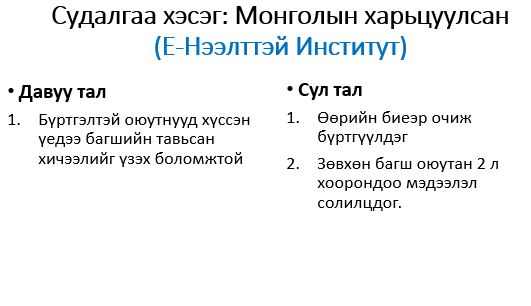
\includegraphics[width=\textwidth]{mongolsudalgaa}
   {И-Нээлттэй институт}
   
    Эрхэм зорилго
        Боловсролын хэрэгцээг орон зай, цаг хугацаанаас төдийлөн шалтгаалахгүйгээр уян хатан, олон хувилбартай, нээлттэй, хүртээмжтэй, чанартай, үр ашигтайгаар хангах нээлттэй боловсролын тогтолцоог бий болгоход оршино.
        
    АЛСЫН ХАРАА
        Дэлхий нийтийн нээлттэй боловсролын сүлжээнд өөрийн байр суурь, нэр хүнд бүхий Монголын нээлттэй их сургууль болж улмаар дэлхийн мэдлэг мэдээллийн охийг Монголд, Монголын чадварлаг залуусыг дэлхийд таниулахад бодит хувь нэмэр оруулна.
        
    
    Е-Нээлттэй Институтийн Түүх
       Манай улсад ерээд оны дундуур орчин үеийн интернетийн технологи анх орж ирснээр байгууллагын төрөлжсөн болоод улсын хэмжээний нэгдсэн сүлжээ байгуулах эхлэл тавигдсан билээ. Үүнтэй уялдаж тодорхой боловсрол эзэмшсэн хүмүүст компьютерийн мэдлэг олгох, бүх шатны сургалтанд компьютерын техник нэвтрүүлэх, мэдээллийн технологийн хичээл заах, улсын хэмжээнд үйл ажиллагаандаа тооцоолох техникийг өргөн ашигладаг болох, холбогдох програм хангамжийг боловсруулах ажил өрнөсөн юм. Энэхүү улсын хэмжээний асуудлыг шийдвэрлэхэд манай их сургуулийн бүрэлдэхүүний Компьютерийн техник менежментийн сургууль (КТМС), Холбоо мэдээллийн сургууль (ХМС) тус тус томоохон үүрэг гүйцэтгэсний дотор системийн програм хангамж боловсруулах, байгууллагын дотоод ба системийн түвшний сүлжээ байгуулах, мэргэжлийн боловсон хүчин бэлтгэх, гадаад орнуудтай хамтран ажиллах, шинжлэх ухааны ололт амжилт, тэргүүн туршлагаас суралцаж, их сургуулийн үйл ажиллагаанд нэвтрүүлэх зэрэг олон чиглэлийн ажлыг ректор Д.Бадарчийн удирдлагын дор мэргэжлийн баг амжилттай гүйцэтгэж ажилласнаар тодорхой хүрсэн үр дүнгийн нэг тод илрэл бол ирээдүйн нээлттэй судалгааны Шинжлэх Ухаан, Технологийн Их Сургуулийн үндэс суурь болсон Е-Нээлттэй сургуулийг 2010 онд БСШУ-ны Сайдын 2007 оны 6 дугаар сарын 5-ны өдрийн 183 тоот тушаалын 6 дугаар зүйлд заасны дагуу дотоодын их сургууль, коллежийн зайн сургалтыг хариуцуулахаар ШУТИС-ийн бүрэлдэхүүнд байгуулсан явдал юм.
	\subsection{Гадаадын системүүдийн харьцуулсан судалгаа}
	
	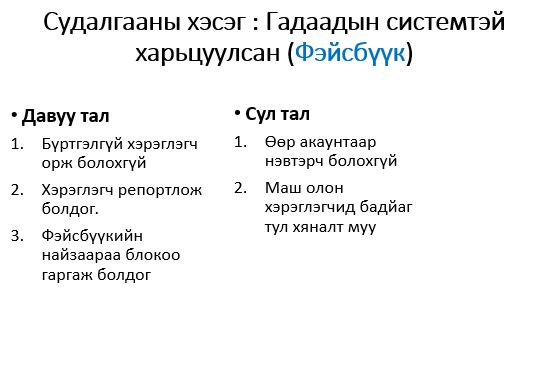
\includegraphics[width=\textwidth]{gadaadsudalgaa}

	
	\subsection{Хууль, дүрэм журам}
	2010 онд БСШУ-ны Сайдын 2007 оны 6 дугаар сарын 5-ны өдрийн 183 тоот тушаалын 6 дугаар зүйлд заасны дагуу дотоодын их сургууль, коллежийн зайн сургалт явуулж болно. 
	
	
	\section{Технологийн судалгаа}
	
	\subsection{Laravel фреймворк}
	Ларавел фреймворк нь  MVC вэб програмуудын хөгужилд зориулагдсан үнэгүй, нээлттэй эхтэй PHP вэб фреймворк юм. Ларавел нь MIT тусгай зөвшөөрөлтэй бөгөөд GitHub дээр байршдаг. PHP орчинд алдартай 2013 оны 12 сарын судалгаагаар Laravel  2014 оны хувьд хамгийн ирээдүйтэй PHP вэб фреймворк гэж судлагдсан байдаг.
	PHP фреймворкүүдийг 2015 оны эцсийн байдлаар харьцуулж үзэхэд  хамгийн их хэрэглэгддэг фреймворк гэдэг нь судалгаагаар тогтоогдсон.
	
	\subsection{MySQL}
	MySQL нь холбоост өгөгдлийн санг удирдах систем юм. MySQL хэмээх нэрний хувьд уг системийг санаачлан хөгжүүлэгч Micheal Widenius-ын охины нэр My + SQL(Structed Query Language) гэсэн утгатай ажээ.
	Энэ систем нь GNU (General Public License) буюу нээлтэй эхийн систем учир хүссэн хэн бүхэн хөгжүүлэлтэнд оролцож, үнэгүй хэрэглэж болох юм. Эзэмшигч нь алдарт Java-г хөгжүүлсэн Sun MicroSystems компани байсан ба, одоогоор Sun-г Oracle корпораци эзэмших болсон билээ.
	Үнэгүй програм хангамжийн өгөгдлийн санг удирдах системд ихэвчлэн MySQL-ийг хэрэглэдэг бөгөөд тэдгээрийн сонгодог жишээ гэвэл Joomla, Drupal, Wordpress, phpBB гэх мэт агуулга удирдах системүүд (CMS-Content Management System), Wikipedia, Facebook, Google гэх мэт томоохон компаниуд хэрэглэдэг юм.
	Хөгжүүлэлт нь C/C++ хэл дээр хийгдсэн ба AIX, BSDi, FreeBSD, HP-UX, i5/OS, Linux, Mac OS X, NetBSD, Novell NetWare, OpenBSD, OpenSolaris, eComStation, OS/2 Warp, QNX, IRIX, Solaris, Symbian, SunOS, SCO OpenServer, SCO UnixWare, Sanos, Tru64, Microsoft Windows гэсэн олон үйлдлийн системүүд дээр ажилладаг.
	MySQL бол хамгийн өргөн хэрэглээтэй нээлттэй эхийн (Open Source) өгөгдлийн сан удирдах програм юм. Анх 1995 онд зах зээлд гарсан ба с/с++ хэл дээр бичигдсэн. Одоогийн байдлаар 5.7 нь хамгийн сүүлийн хувилбар болон гараад байна. Энэ сүүлийн хувилбар дээр нэмэгдсэн давуу талууд гэвэл 3 дахин хурдан үйл ажиллагаатай болсон мөн натив JSON дэмжигчтэй болсон гэх мэт шинэлэг үйлдлүүд нэмэгдсэн байна.
	
	\subsection{Php}
	Rasmus Lerdorf WWW-д вэб хуудас үүсгэх үедээ өгөгдөл боловсруулах хялбархан арга хайж байгаад 1995 онд PHP хэлийг скрипт хэл байдлаар зохиосон.
	PHP нь сервер талын скрипт хэл ба динамик вэб хуудас хийхэд илүү тохиромжтой. Энэ скрипт хэл нь энгийн хэрэглээний вэб сайтаас эхлээд байгууллагын иж бүрэн вэб программ хийж болохоор MySQL мэтийн өгөгдлийн сантай харилцан ажиллах боломжтой.
	Хуудас ачаалах үед броузерээр нэг бүрчлэн уншдаг HTML-тэй адилгүй, PHP баримтыг бэлтгэхдээ серверээр урьдчилан боловсруулдаг. PHP код агуулсан хуудас нь хэрэглэгчийн броузерт илгээгдхээс өмнө серверээр боловсруулагдсан байдаг.
	PHP хэлний өөр нэг давуу тал бол скриптэн хэл юм. Ихэнх програмчлалын хэлнүүдэд ажиллахын өмнө машины хэл рүү хөрвүүлэх тусгай файлууд /compile/ шаардлагатай байдаг бол PHP хэлний хувьд хөрвүүлэлт хийх шаардлагагүй байдаг тул код засварлах болон шалгахад илүү хурдан байдаг
			\subsection{SQL injection (тарилга) гэж юу вэ? }
		SQL injection бол ӨС-ийнхамгийн том аюул заналуудын нэг .
		ӨС эсвэл Вэб апп-ийн front-end-ээр дамжуулан өгөгдийн санруу хандах үйл ажиллагаа
		SQL injection нь Вэб апп –ууд дээр өргөн тохиолддог бөгөөд SQL injection –г ашишлахад амар байдаг.
		Тийм учираас ӨС-руу хандахад илүү өргөн ашиглагддаг.
		SQL injection нь ӨС дээр query-г гүйцэтгэхийн өмнө query-нд шүүгээгүй утга эсвэл вэб апп-ийн input талбар дээр хортой хавсаргаад ажиллуулах үед тохиолддог. 
		1. Үүний үр дүнд дараахм боломжууд үүсдэг.
		2. Чухал мэдээлэлд (sensitive data)-д хандах
		3. Илүү аюултай exploit хийх
		ӨС байгаа сервер, үйлдлийн систем дээр команд гүйцэтгэх
		
		\subsection{Эрхийг өргөжүүлэх (privilege escalation) халдлага гэж юу вэ? }	
		Privilege escalation буюу эрхийг өргөтгөх нь аюултай аюул ганал юм. 
		Privilege escalation-ийн боломжоос хамааран хортой нэмэлт нэмэх, өгөгдлийн өөрчлөх, устгах боломж олгож байгууллагыг хүнд бадйлд сүрэлд оруулдаг юм.
		
		
		\subsection{Үйлчилгээг зогсоох (DoS – Denial of Service) халдлага гэж юу вэ?}
		Denial of Service эсвэл Dos халдлага нь buffer overflow хийх, data corruption хийх эсвэл серверийн бусад нөөцийг ашиглах бадлаар үүсдэг. 
		Dos халддлага нь серверийг унагааж өгөгдлийн санг холбогдоох боломжгүй (unreachable болгодог ба халдлага удаан үргэлжилж болно.
		
		\subsection{Black box тест гэж юу вэ?}
		Black box тестд ӨС-ийн нэгдсэн баталгаажуулалт, функционал шалгалт хамаардаг. Шалгах кейсүүд нь энгийн бөгөөд үйл ажиллагаанаас ирж байгаа болон гарж байгаа өгөгдлийг баталгаажуулахад ашигладаг.
	\newpage
	\section{Шинжилгээ, зохиомжийн хэсэг}
	\subsection{Функциональ шаардлага}
	\paragraph {Хэрэглэгч (Багш, Оюутан, Эцэг эх)}
	\begin{itemize}
		
	\item Нэвтрэх (Имэйл эсвэл утас оруулах нууц үг оруулах )
	\item Бүртгүүлэх (Овог, нэр, имэйл эсвэл утас, нууц үг) бөглөх
	\item Нууц үг сэргээх (Имэйл эсвэл утас бичээд өгөгдсөн тэдэгтийг оруулах)
	\item Фэйсбүүкээр нэвтрэх 
	\item Gmail-ээр нэвтрэх
	\item Блок арилгах (зургаар таниж блок гаргах, бичиг баримтны зургаар гаргах, утас/ имэйлээр блок гаргах )
	
     \end{itemize}
     \paragraph {Админ}
     \begin{itemize}
 	
 	\item Нэвтрэх ( Нэрээ оруулах нууц үг оруулах )
 	\item Бүртгэх
 	\item Репортуудын жагсаалт харах
 	\item Хэрэглэгчийг нэрээр хайх
 	\item Хэрэглэгчийг блоклох
 	\item Хэрэглэгчийг устгах
 
 	
    \end{itemize}
	\subsection{Функциональ бус шаардлага}
	\begin{itemize}
		\item Хэрэглэхэд хялбар ойлгомжтой, дэлгэрэнгүй байх
		\item Мэдээллийг түргэн шуурхай харуулдаг байх
		\item Алдааны мэдээлэл өгдөг байх 
		\item Бүх төрлийн төхөөрөмжид тохиромтой хэлбэрээр харагддаг /респонсив/ загвартай байна
	\end{itemize}
	\section{Юзкейс диаграм}
	\subsection{Админы юзкейс диаграм}
     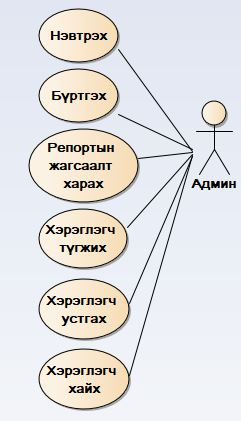
\includegraphics[width=\textwidth]{adminUseCase}
	\subsection{Хэрэглэгчийн юзкейс диаграм}
     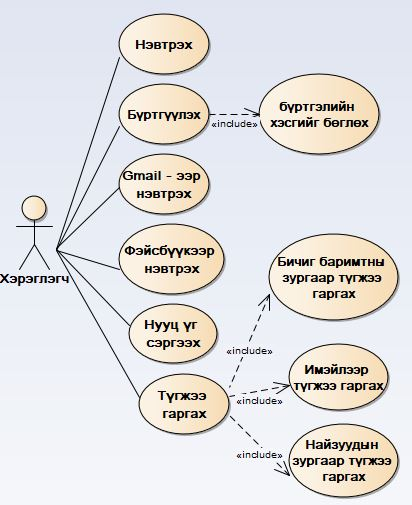
\includegraphics[width=\textwidth]{userUseCase}
     	\section{Интерфэйс}
     	\subsection{Нэвтрэх хэсгийн интерфэйс}
     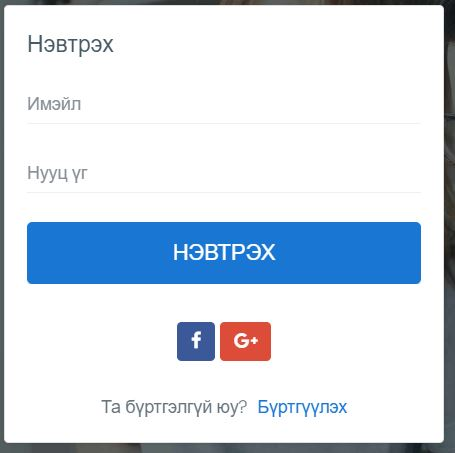
\includegraphics[width=\textwidth]{login}
     \subsection{Бүртгүүлэх хэсгийн интерфэйс}
     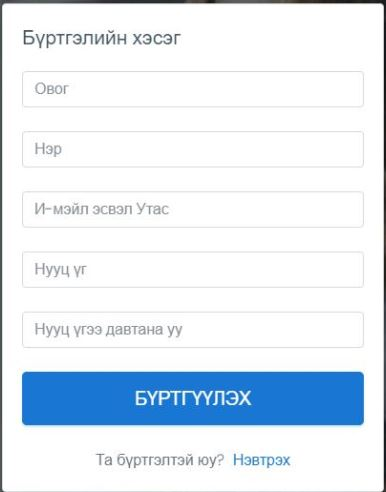
\includegraphics[width=\textwidth]{delgets}
     \subsection{Админы интерфэйс}
     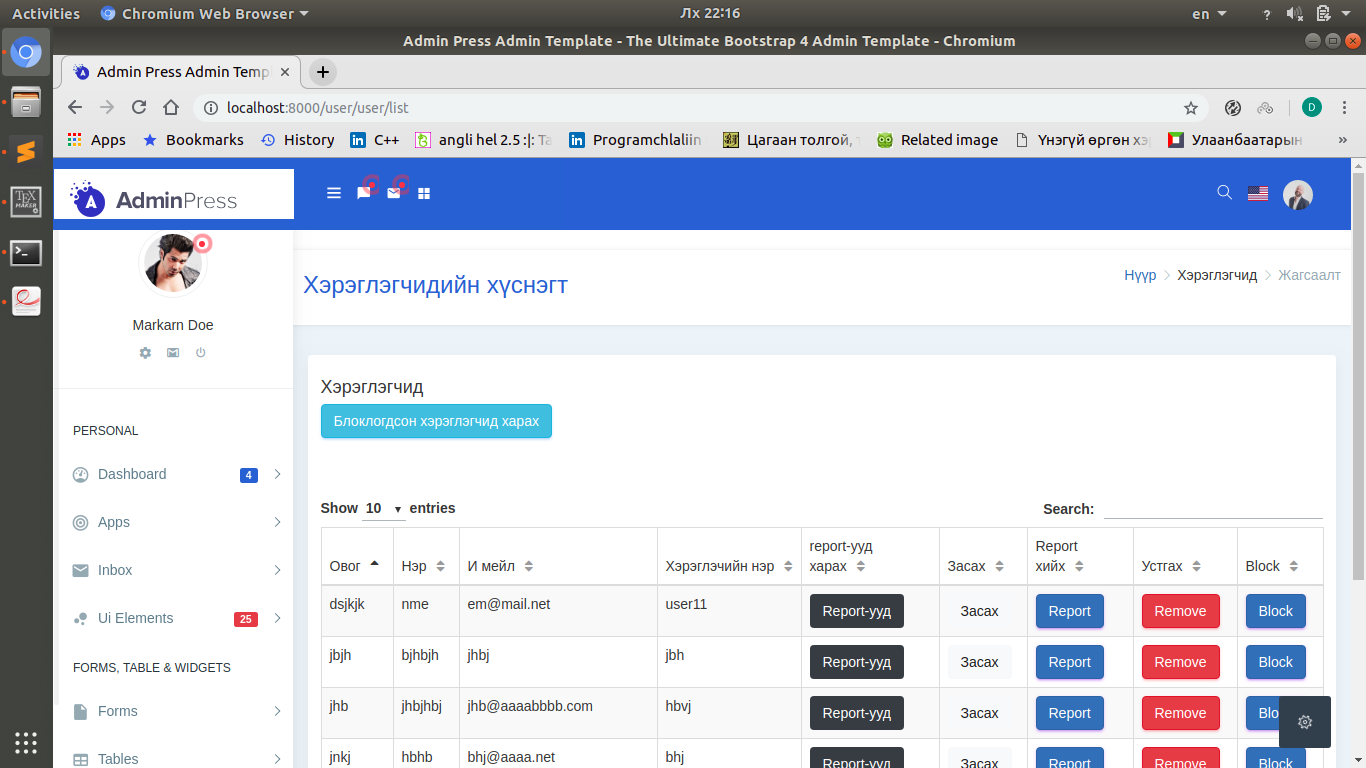
\includegraphics[width=\textwidth]{delgets1}
      \subsection{Репортлох интерфэйс}
     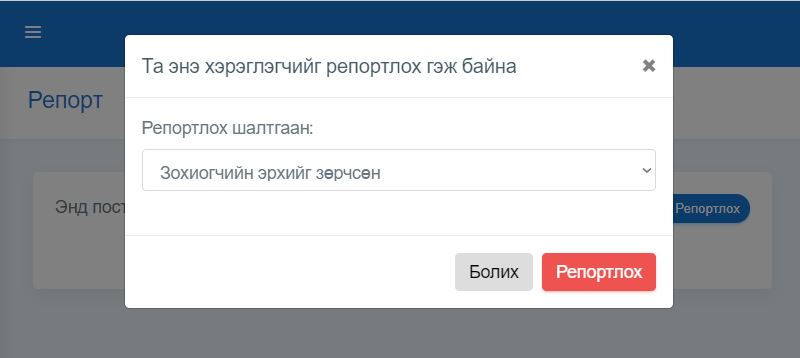
\includegraphics[width=\textwidth]{delgets2}
     	
     	\section{Үйл ажиллагааны диаграм}
     	\subsection{Бүртгүүлэх үйл ажиллагааны диаграм}
     	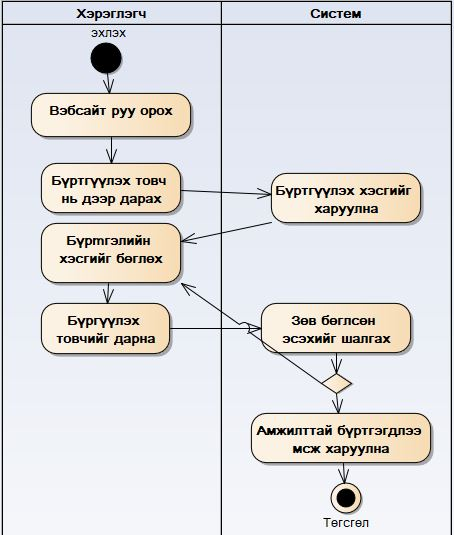
\includegraphics[width=\textwidth]{regActivity}
     	\subsection{Нэвтрэх үйл ажиллагааны диаграм}
     	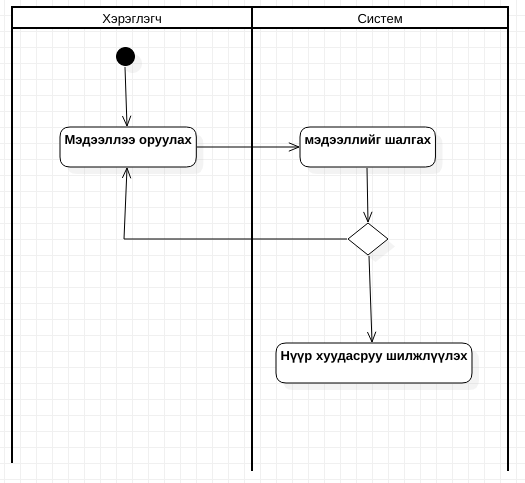
\includegraphics[width=\textwidth]{loginActivity}
     	\subsection{Хэрэглэгч түгжих үйл ажиллагааны диаграм}
     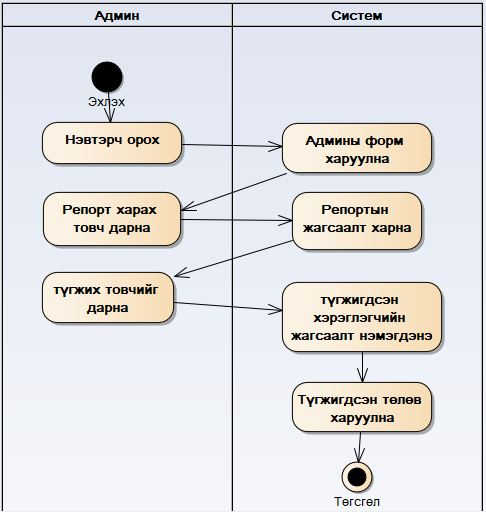
\includegraphics[width=\textwidth]{tugjihActivity}
     \section{Хэрэглэгч түгжээгээ тайлах үйл ажиллагааны диаграм}
     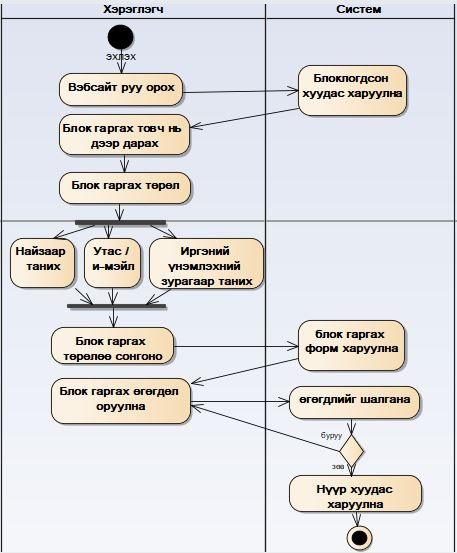
\includegraphics[width=\textwidth]{unblockActivity}
     \section{Обьектын холбоосын диаграмм ( ERD )}
     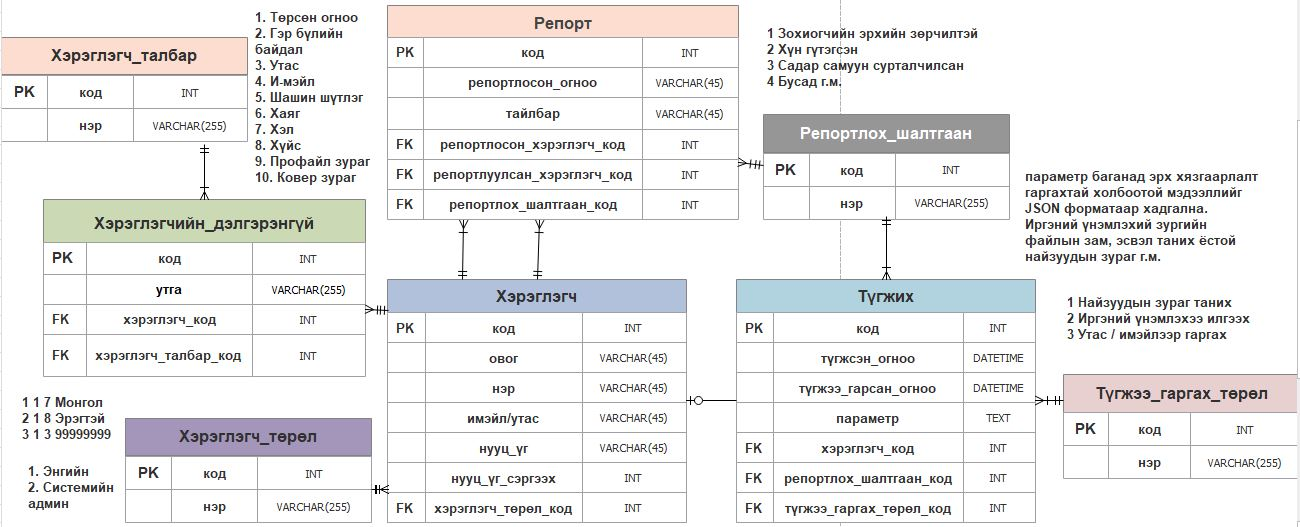
\includegraphics[width=\textwidth]{ERDagram}
      \section{Класс диаграм ( Class diagram )}
     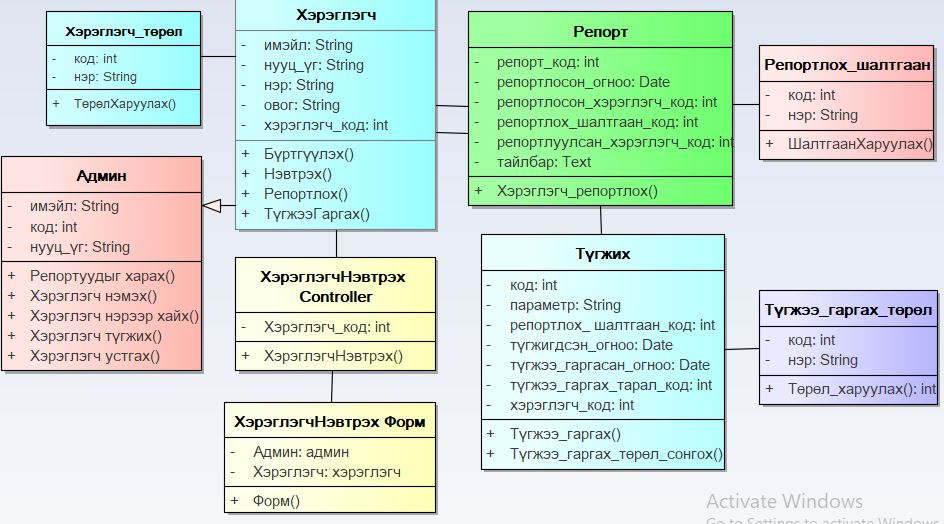
\includegraphics[width=\textwidth]{class}
     \section{Дараалалын диаграмм( Sequence diagram )}
           \subsection{Хэрэглэгч бүртгэх дараалалын диаграм}
     \includegraphics[width=\textwidth]{addsequence	11	}
     \subsection{Хэрэглэгч түгжих дараалалын диаграм}
     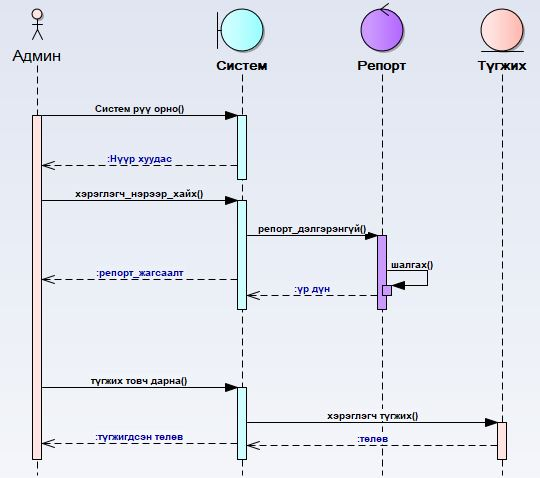
\includegraphics[width=\textwidth]{sequence1}
      \section{Төлөвийн диаграм }
     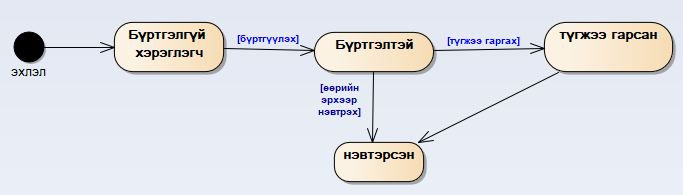
\includegraphics[width=\textwidth]{statechartDiagram}
     \section{Юзкейз тодорхойлолт }
      \subsection{Бүртгүүлэх юзкейз тодорхойлолт }
     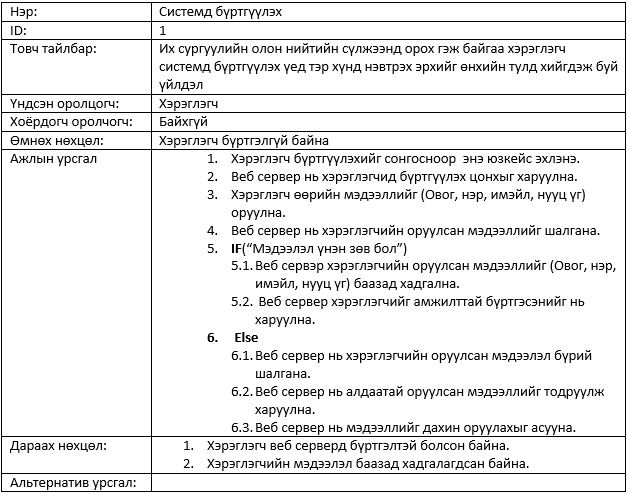
\includegraphics[width=\textwidth]{usecaseT}
      \subsection{Хайлт хийх юзкейз тодорхойлолт}
     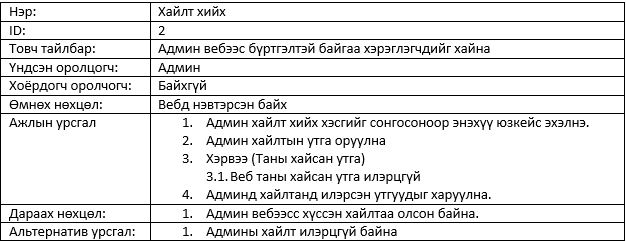
\includegraphics[width=\textwidth]{usecaseT2}
     \subsection{Хэрэглэгч репортлох юзкейз тодорхойлолт }
     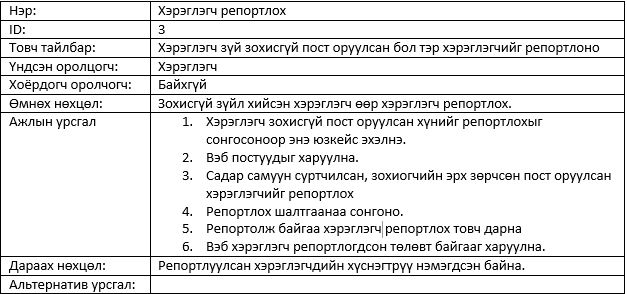
\includegraphics[width=\textwidth]{usecaseT3}
     \subsection{Хэрэглэгч түгжих юзкейз тодорхойлолт}
     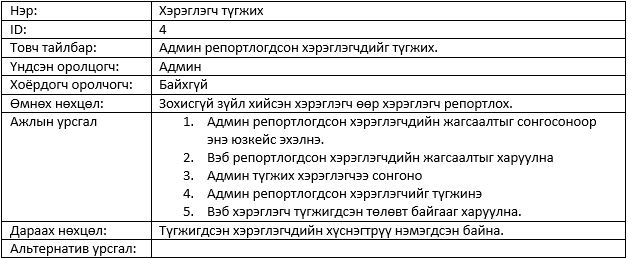
\includegraphics[width=\textwidth]{usecaseT4}
     \subsection{Бүртгэлтэй хэрэглэгч харах юзкейз тодорхойлолт }
     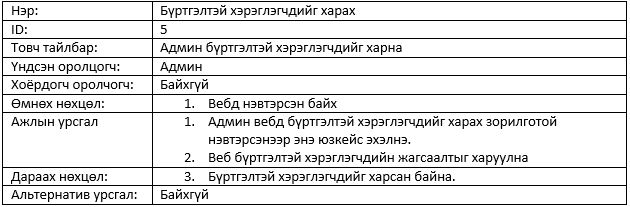
\includegraphics[width=\textwidth]{usecaseT5}
     \subsection{Нэвтрэх юзкейз тодорхойлолт}
     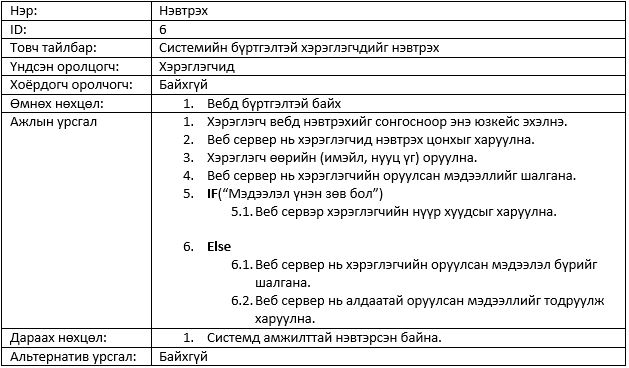
\includegraphics[width=\textwidth]{usecaseT6}
     
     \section{Дүгнэлт}
     Хамгийн гол нь үнэн зөв мэдэглэгийг олж авах тиймээс Их сургуулийн олон нийтийн сүлжээ нь хэрэглэгчид сайтад оюуны өмчийг зөрчиж байгаа болоод ёс бус мэдээлэл тавьж буй хүмүүсийг репортолж тэдгээр хэрэглэгчидийг түгжих гэх мэт аргаар болиулах шаардлагатай  байна. Мөн системрүү хадлага хийх гэж оролдох тохиолдолд түүнээс хамгаалсан ёстой.
    
     
     \section{Ашигласан бүтээлийн жагсаалт}
     \subsection{Ном зүй}
     \subsection{Вэб сайтууд}
     http://www.schoolweb.mn/schools/
     
     http://www.meds.gov.mn/data/said/Боловсрол%20Эрх%20зүйн%20баримт%20бичиг.pdf
     
\end{document}



